
\begin{frame}[fragile]{Qu'est-ce que la normalisation}

La \alert{normalisation} relationnelle consiste à élaborer
un schéma de données avec deux propriétés fondamentales\;:

\vfill 

\begin{redbullet}
  \item Il n'y a \alert{aucune} redondance, et donc aucun risque \alert{d'incohérence}
  \item Il n'y a aucune \alert{perte d'information}
\end{redbullet}

\vfill


\begin{noteblock}
Essentiel pour les bases de données généralistes. Beaucoup moins important
pour des données historisées
servant à l'analyse.
\end{noteblock}

\end{frame}




\begin{frame}{Pourquoi pas une unique table\,?}

\begin{small}
\begin{center}
\begin{tabular}{l|c|l|l|l|c}
 date &  nom &  âge & département &  région &  pathologie \\
\hline
12/01/23 & Philippe R. & 63 &Paris & IdF & Diabète\\
05/10/24 & Amélie A. & 32 & Var & PACA & Cancer\\
31/03/22  & Julien S. & 16 & Manche & Normandie & Cardio\\
14/01/24 & François J. &  52 & Orne & Normndie  & Neurologique \\
02/07/21 & Sonia T. & 38 & Paris & Ile de F. & Diabète \\
25/06/22 & Philippe R. & 25 &Cantal  & ARA  &  Respiratoires\\
03/12/24 & Joëlle B.  & 72 & &  & Cardiologiques\\
27/04/22  & Sonia T.  & 89 & Var & PACA & Epilespsie\\
\hline
\end{tabular}
\end{center}
\end{small}

\vfill

Enumérons les \alert{anomalies}  (insertion, modification, suppression)
et \alert{incohérences}.
\end{frame}



\begin{frame}{Petit résumé}

Une liste (non exhaustive) des problèmes soulevés par
une modélisation bâclée.

\vfill
\begin{redbullet}
  \item Impossible d'identifier des patients, régions ou pathologies
  \item Pas de regroupement possible, pas d'agrégation fiable
     \item Pas de nomenclature des pathologies sans patient -- pas
         de répertoire des patients sans pathologie
   \item Un même patient peut voir ses propriétés varier -- deux
      patients disctincts peuvent être indiscernables
    \item etc.
\end{redbullet}


\end{frame}


\begin{frame}{Qu'est-ce que normaliser\,?}

La normalisation consiste à 
\vfill
\begin{redbullet}
  \item distinguer des ``entités'' 
  \item les identifier 
     \item leur affecter une table spécifique 
   \item lier ces tables pour ne pas perdre d'information
\end{redbullet}

\vfill


\begin{noteblock}
Il existe des méthodes et des propriétés formelles pour dire 
qu'un schéma est normalisé. Cf un cours sur les BD relationnelles.
\end{noteblock}

\end{frame}

\begin{frame}{La modélisation de notre schéma}



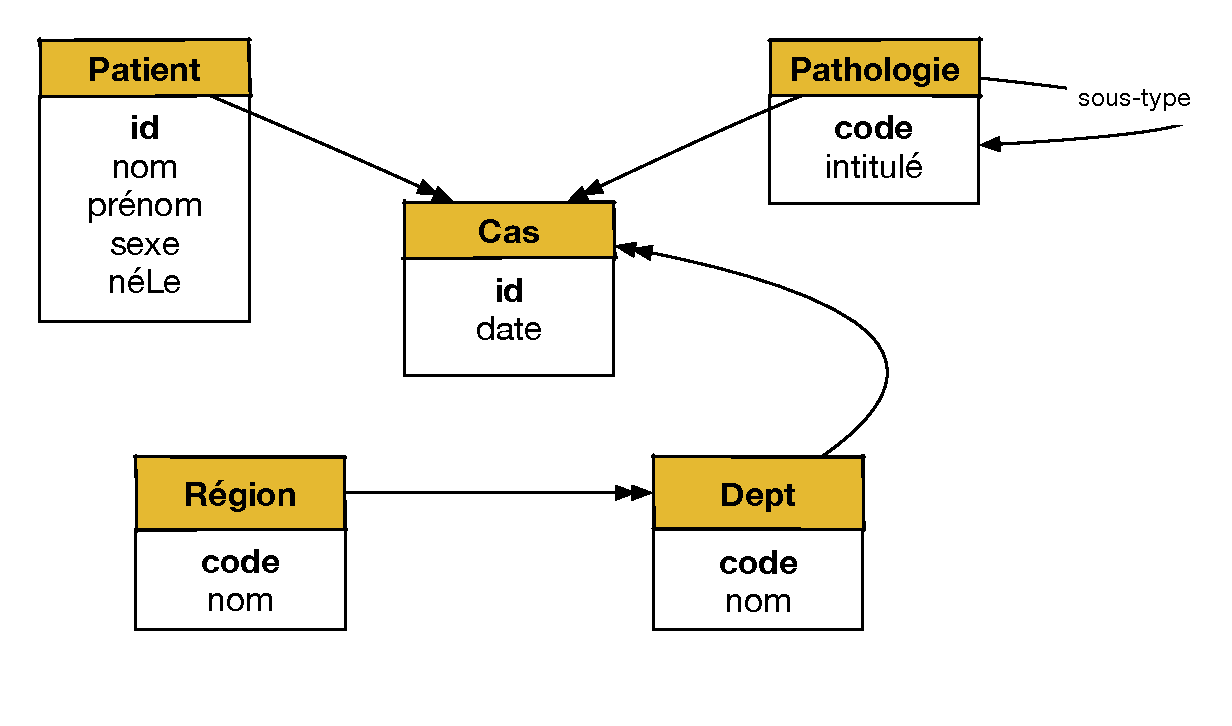
\includegraphics[width=1\textwidth]{../figures/cs103_modele}


\end{frame}

\begin{frame}{Les bases OLAP}

Notre schéma est ``en étoile'', caratéristique des entrepôts de données.
Des \alert{faits} (ici des cas) sont qualifiés selon plusieurs 
\alert{dimensions}, parfois hiérarchiques.

\vfill

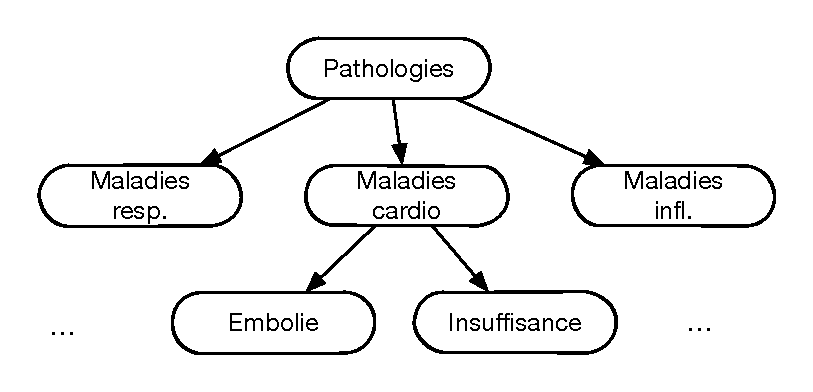
\includegraphics[width=0.6\textwidth]{../figures/cs103_pathos}

\vfill

L'opération de \alert{rollup} permet de se placer à différents niveaux 
de la hiérarchie.
\end{frame}


\begin{frame}{Nos tables}


En \textbf{gras} les \alert{clés primaires}, en \textit{italiques} les
\alert{clés étrangères}.

\vfill

\begin{redbullet}
  \item Patient (\textbf{id}, nom, prénom, sexe, néLe)
  \item Pathologie (\textbf{code}, intitulé, \textit{sousTypeDe})
  \item Région (\textbf{code}, nom)
  \item Dépt (\textbf{code}, nom, \textit{codeRégion})
  \item Cas (\textbf{id}, date, \textit{idPatient}, \textit{codePathologie}, \textit{codeDépt})
\end{redbullet}

\vfill

Voir \url{https://deptfod.cnam.fr/bd/tp}
\end{frame}

%%%%%%%%%%%%%%%
\begin{frame}{Le mécanisme des clés primaires et étrangères}
 

\begin{minipage}[t]{7cm}
\begin{tabular}{c|p{5cm}}
\textbf{code} & nom \\ \hline
 paca  & Provence, Alpes, Côte d'azur\\
ara & Auvergne, Rhône Alpes\\
nmd & Normandie\\
occ & Occitanie\\
\hline
\end{tabular}
La table des régions
\end{minipage} \
\begin{minipage}[t]{5cm}


\begin{tabular}{c|c|c}
\textbf{code} & nom & \textit{codeRégion} \\ \hline
 15  & Cantal & ara \\
50 & Manche & nmd\\
30 & Gard & occ\\
61 & Orne & nmd
\\
\hline
\end{tabular}
La table des départements
\end{minipage}

\vfill

\begin{remblock}{Contraintes}
\begin{redbullet}
  \item la valeur d'une clé primaire est unique (pas de doublon)
 \item La valeur d'une clé étrangère est \alert{toujours} celle
d'une clé de la table référencée (\emph{intégrité référentielle})
\end{redbullet}
\end{remblock}
\end{frame}

%%%%%%%%%%%%%%%
\begin{frame}{Suite et fin des exemples}
 

\begin{minipage}[t]{7cm}
\begin{tabular}{c|c|c|c}
\textbf{id} & prénom & sexe & néLe \\ \hline
 10  &  Philippe & M & 18/09/1987\\
20 & Amélie & F & 12/01/1963\\
30 &Julien & M & 2/11/2002\\
40 & François & M & 30/03/1993\\
50 & Joëlle & F & 18/02/1997\\
60 & Sonia & F & 29/07/1976\\
\hline
\end{tabular}

La table des patients
\end{minipage} \hspace*{2mm} \
\begin{minipage}[t]{5cm}
\begin{tabular}{c|c|c}
\textbf{code} & intitulé & \textit{sousTypeDe} \\ \hline
dia  & Diabètes &  \\
neur & Neurologies & \\
canc & Cancers & \\
epi & Epislespie & neur \\
csein & Cancer du sein & canc\\
psy & Psychiatrie & \\
\hline
\end{tabular}
La table des pathologies
\end{minipage}

\vfill
\begin{center}
\begin{tabular}{c|c|c|c|c}
\textbf{id} & date & idPatient & codePathologie & codeDépt \\ \hline
1000  & 08/12/2021 & 10 & epi & 30\\
2000 &  24/05/2024 & 40 & dia & 15\\
3000 &  30/03/2021 & 50 & epi & 30\\
4000 &  18/07/2022 & 10 & neur & 61\\
5000 &  06/10/2021 & 20 & csein & 61\\
6000 &  20/07/2023 & 60 & dia & 50\\
\hline
\end{tabular}
La table des cas
\end{center} 
\end{frame}


%%%%%%ù

\begin{frame}{À retenir}

Un modèle relationnel normalisé évite les \alert{anomalies de mise à jour} et
les \alert{incohérences}.
\vfill
Caractéristiques\,:

\begin{redbullet}
  \item La base est constitué de plusieurs (souvent, beaucoup) de tables
      contenant des données élémentaires
 \item Les liens sont basés sur les partages de valeur (clés primaire et étrangère)
 \item L'ajout d'une information (un cas par exemple) peut nécessiter 
        plusieurs écritures
 \item La recherche d'une information peut nécessiter plusieurs lectures
 \item Toutes les données sont ``à plat'', aucun accès n'est privilégié
\end{redbullet}

\vfill

\alert{A-t-on perdu de l'information}\,? Comment reconstituer la table ``universelle'' 
avant décomposition\,? À venir.
\end{frame}



\begin{frame}{La pratique}

Les données disponibles en Open Data sont le plus souvent agrégées, sans doute
à partir d'une base relationnelle sous-jacente.

\vfill

Défi\,: choisissez un jeu de données et proposez une modélisation
des faits élémentaires.

\vfill

Exemples
\begin{redbullet}
  \item Le modèle proposé est inspiré de \url{https://data.ameli.fr/explore/?refine.theme=Pathologies}
  \item Sur le même site vous pouvez prendre les montants des honoraires 
  des professionnels de santé et modéliser une base ``Consultations''.
  \item Le choix du jeu de données est libre\,!
\end{redbullet}

\end{frame}
